\subsection{Monitoring}
\label{section:process-monitoring}
We chose to monitor the number of requests and request latency for each endpoint on our server, and we monitored the CPU and memory usage of it. We chose these because they give a quick overview of how the system is performing and because they allow us to diagnose issues faster, by locating when something happened, at which endpoint and if it had an effect on system resources.

As an example, we used the request latency to add SQL indexes to our database, as we had some slow endpoints. For a different example where we had an issue with our system, which was reflected in the monitoring, see \appendixref{appendix:monitoring-samples}.

\begin{figure}[H]
    \makebox[\textwidth][c]{
        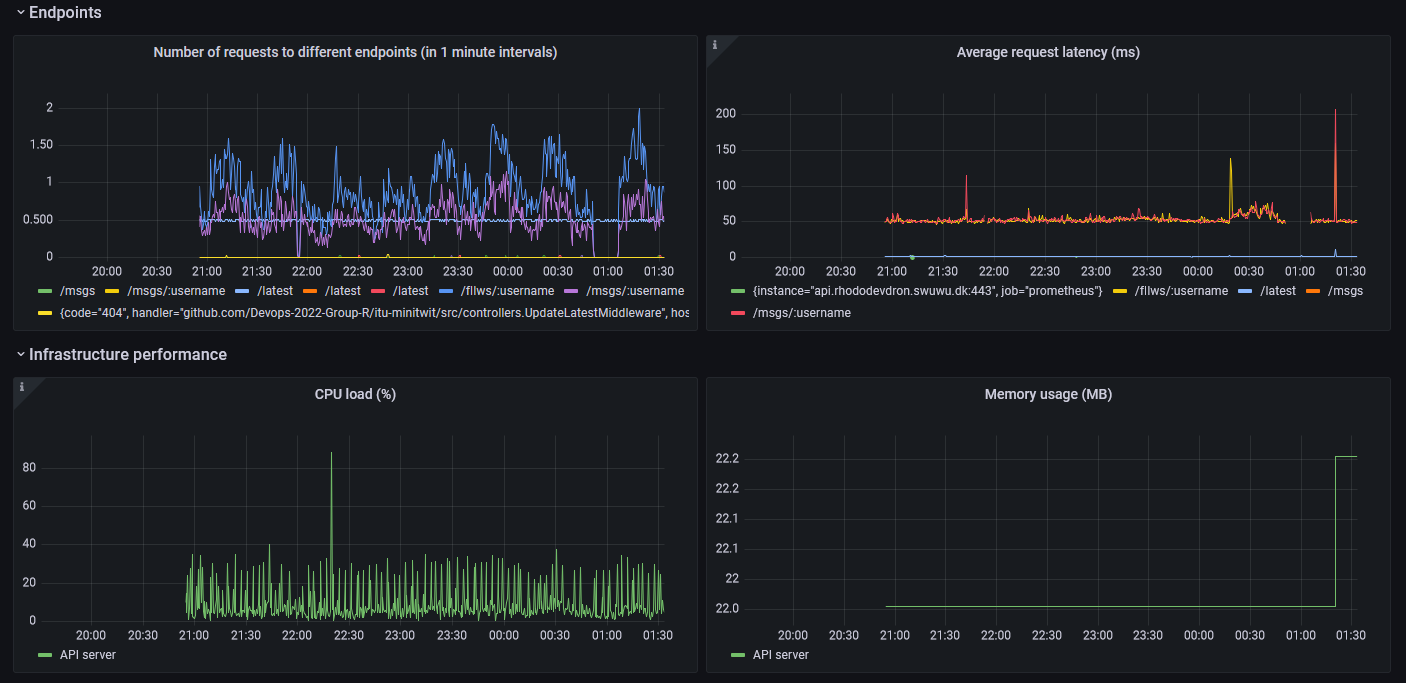
\includegraphics[width=0.85\paperwidth]{grafana-dashboard}
    }%
    \caption{A sample of our Grafana dashboard.}
\end{figure}
